\documentclass[11pt,a4paper]{article}
\usepackage[margin=1in]{geometry}
\usepackage{graphicx}
\usepackage{tabularx}
\usepackage{longtable}
\usepackage{array}
\usepackage{booktabs}
\usepackage{xcolor}
\usepackage{colortbl}
\usepackage{fancyhdr}
\usepackage{titlesec}
\usepackage{enumitem}
\usepackage{tikz}
\usepackage{tikz-timing}
\usetikzlibrary{positioning,arrows,shapes,automata}
\usepackage{amsmath}
\usepackage{listings}
\usepackage{multirow}
\usepackage{adjustbox}

% Define colors
\definecolor{darkblue}{RGB}{25,25,112}
\definecolor{darkgreen}{RGB}{0,100,0}
\definecolor{darkred}{RGB}{139,0,0}

% Custom section formatting
\titleformat{\section}{\Large\bfseries\color{darkblue}}{\thesection}{1em}{}
\titleformat{\subsection}{\large\bfseries\color{darkgreen}}{\thesubsection}{1em}{}
\titleformat{\subsubsection}{\normalsize\bfseries}{\thesubsubsection}{1em}{}

% Header and footer
\pagestyle{fancy}
\fancyhf{}
\fancyhead[L]{Mandelbrot Fractal Generator}
\fancyhead[R]{ECE298A - August 2025}
\fancyfoot[C]{\thepage}

\begin{document}

% Title page
\begin{titlepage}
\centering
{\Huge\bfseries\color{darkblue} Mandelbrot Fractal Generator\\[0.5cm]}
{\Large\bfseries Hardware Design Document\\[2cm]}

\begin{tabular}{ll}
\textbf{Authors:} & Taisir Hassan, Evan McCarthy \\[0.3cm]
\textbf{Course:} & ECE298A \\[0.3cm]
\textbf{Document Version:} & 1.0 \\[0.3cm]
\textbf{Date:} & August 2025 \\[0.3cm]
\textbf{Target Platform:} & TinyTapeout \\[0.3cm]
\textbf{Technology Node:} & Sky130 (130nm) \\[0.3cm]
\textbf{Design Language:} & SystemVerilog \\[0.3cm]
\textbf{Verification:} & Cocotb Python Testbench \\[0.3cm]
\end{tabular}

\vfill
\end{titlepage}

% Table of Contents
\tableofcontents
\newpage

\section{Executive Summary}

\subsection{Project Objective}
This document specifies the design and implementation of a real-time Mandelbrot fractal generator optimised for the TinyTapeout ASIC platform. The system generates mathematically accurate fractal visualisations using hardware-accelerated fixed-point arithmetic, targeting 640×480 VGA display output at 60Hz refresh rate.

\subsection{Key Features}
\begin{itemize}
\item Real-time fractal computation at 25MHz pixel rate
\item Dual clock domain architecture (50MHz system, 25MHz VGA)
\item Q3.8 fixed-point arithmetic for area-optimised implementation
\item Interactive zoom and pan functionality
\item Multiple colour mapping schemes (4 modes)
\item TinyTapeout-compliant I/O interface
\item Comprehensive verification testbench suite
\end{itemize}

\subsection{Technical Specifications}
\begin{table}[h]
\centering
\begin{tabularx}{\textwidth}{|l|X|l|}
\hline
\rowcolor{darkblue!20}
\textbf{Parameter} & \textbf{Specification} & \textbf{Unit} \\
\hline
Display Resolution & 640 × 480 & pixels \\
Refresh Rate & 60 & Hz \\
Pixel Clock & 25 & MHz \\
System Clock & 50 & MHz \\
Colour Depth & 6-bit RGB & 64 colours \\
Arithmetic Format & Q3.8 Fixed Point & 11-bit signed \\
Maximum Iterations & 64 & iterations \\
Power Consumption & $<$10 (estimated) & mW \\
Technology Node & Sky130 & 130nm \\
\hline
\end{tabularx}
\caption{System Technical Specifications}
\end{table}

\newpage
\section{System Overview}

\subsection{System Architecture}
The Mandelbrot fractal generator implements a pipelined architecture with dedicated modules for computation, display timing, colour mapping, and parameter control. The system processes one pixel per clock cycle, achieving real-time fractal generation for interactive exploration.

\subsection{Functional Block Diagram}
\begin{figure}[h]
\centering
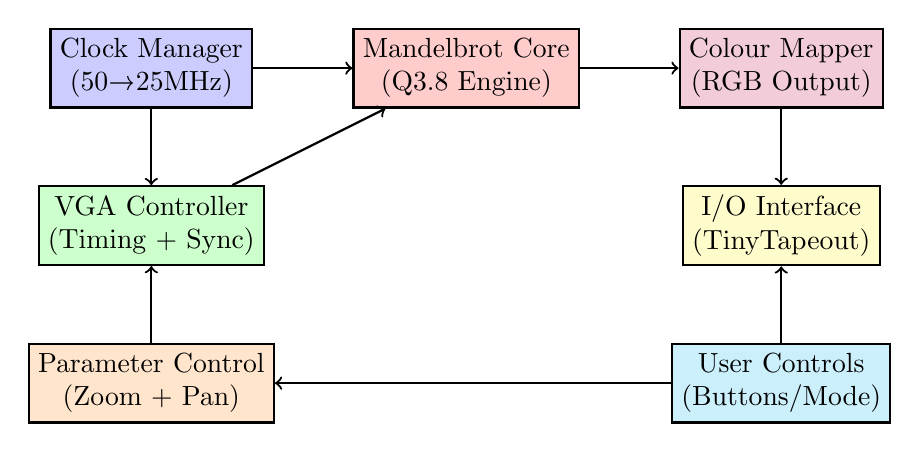
\begin{tikzpicture}[
  block/.style={rectangle, draw=black, thick, minimum width=2.5cm, minimum height=1cm, align=center},
  arrow/.style={->, thick}
]

% Top row
\node[block, fill=blue!20] (clk) at (0,4) {Clock Manager\\(50→25MHz)};
\node[block, fill=red!20] (mandel) at (4,4) {Mandelbrot Core\\(Q3.8 Engine)};
\node[block, fill=purple!20] (color) at (8,4) {Colour Mapper\\(RGB Output)};

% Middle row
\node[block, fill=green!20] (vga) at (0,2) {VGA Controller\\(Timing + Sync)};
\node[block, fill=yellow!20] (io) at (8,2) {I/O Interface\\(TinyTapeout)};

% Bottom row
\node[block, fill=orange!20] (param) at (0,0) {Parameter Control\\(Zoom + Pan)};
\node[block, fill=cyan!20] (user) at (8,0) {User Controls\\(Buttons/Mode)};

% Arrows
\draw[arrow] (clk) -- (mandel);
\draw[arrow] (mandel) -- (color);
\draw[arrow] (clk) -- (vga);
\draw[arrow] (color) -- (io);
\draw[arrow] (vga) -- (mandel);
\draw[arrow] (param) -- (vga);
\draw[arrow] (user) -- (param);
\draw[arrow] (user) -- (io);

\end{tikzpicture}
\caption{System Functional Block Diagram}
\end{figure}

\subsection{Design Methodology}
The design follows industry-standard methodologies including:
\begin{itemize}
\item Modular hierarchical architecture with clear interface boundaries
\item Clock domain crossing analysis and proper synchronisation
\item Fixed-point arithmetic optimisation for ASIC implementation
\item Comprehensive verification-driven development approach
\item Synthesis-aware RTL coding with timing closure considerations
\item Power and area optimisation through algorithmic choices
\end{itemize}

\newpage
\section{Architecture Specification}

\subsection{Clock Domain Architecture}

\subsubsection{Primary Clock Domains}
\begin{table}[h]
\centering
\begin{tabularx}{\textwidth}{|l|l|l|X|}
\hline
\rowcolor{darkgreen!20}
\textbf{Domain} & \textbf{Frequency} & \textbf{Source} & \textbf{Purpose} \\
\hline
clk\_sys & 50 MHz & External Oscillator & System control and parameter updates \\
clk\_vga & 25 MHz & Internal Divider & VGA timing and pixel processing \\
clk\_async & Asynchronous & Button Inputs & User control interface \\
\hline
\end{tabularx}
\caption{Clock Domain Specifications}
\end{table}

\subsubsection{Clock Domain Crossing Strategy}
\begin{itemize}
\item Quasi-static parameter transfer from 50MHz to 25MHz domain
\item Two-stage synchroniser for asynchronous button inputs
\item Gray code counters for multi-bit signal transitions
\item Dedicated reset synchronisers for each clock domain
\end{itemize}

\subsection{Data Path Architecture}
The computation pipeline implements a single-cycle Mandelbrot iteration per pixel, with the following data flow:
\begin{enumerate}
\item Coordinate generation from VGA timing controller
\item Complex coordinate mapping using configurable parameters
\item Mandelbrot iteration computation with escape detection
\item Colour mapping based on iteration count and mode selection
\item RGB output formatting for TinyTapeout VGA interface
\end{enumerate}

\subsubsection{Clock Domain Timing Waveform}
\begin{figure}[h]
\centering
\begin{tikztimingtable}[%
    timing/dslope=0.1,
    timing/lslope=0.1,
    xscale=1.8,yscale=1.1,
    semithick
]
CLK\_50MHz    & 16{C} \\
CLK\_25MHz    & 2{C}2{C}2{C}2{C}2{C}2{C}2{C}2{C} \\
VGA\_Active   & 4L8H4L \\
X\_Coord      & 4D{320}D{321}D{322}D{323}4D{...}4D \\
Mandel\_Iter  & 4D6D{12}2D{25}2D{8}2D \\
RGB\_Out      & 4D6D{R15}2D{G2A}2D{B08}2D \\
\extracode
\begin{pgfonlayer}{background}
\fill [blue!12,opacity=0.4] (4,-6) rectangle (12,1);
\node [anchor=south,font=\small] at (8,1.2) {Active Pixel Region};
\end{pgfonlayer}
\end{tikztimingtable}
\caption{Data Path Timing Diagram showing Mandelbrot Computation Pipeline}
\end{figure}

\newpage
\section{Module Specifications}

\subsection{Top-Level Module: tt\_um\_fractal}

\subsubsection{Module Purpose}
Integration wrapper providing TinyTapeout interface compliance and system-level coordination between all functional blocks.

\subsubsection{Interface Specification}
\begin{table}[h]
\centering
\begin{tabularx}{\textwidth}{|l|l|l|X|}
\hline
\rowcolor{darkblue!20}
\textbf{Signal Name} & \textbf{Direction} & \textbf{Width} & \textbf{Description} \\
\hline
clk & Input & 1 & System clock (50MHz) \\
rst\_n & Input & 1 & Active-low reset \\
ui\_in[7:0] & Input & 8 & User input controls \\
uo\_out[7:0] & Output & 8 & VGA output (RGB + sync) \\
uio\_in[7:0] & Input & 8 & Bidirectional I/O (unused) \\
uio\_out[7:0] & Output & 8 & Bidirectional I/O (unused) \\
uio\_oe[7:0] & Output & 8 & Bidirectional output enable \\
\hline
\end{tabularx}
\caption{Top-Level Module Interface}
\end{table}

\subsection{Mandelbrot Computation Engine}

\subsubsection{Module Purpose}
Implements the core Mandelbrot set algorithm $z = z^2 + c$ with optimised fixed-point arithmetic. Computes escape-time iteration count for each pixel coordinate.

\subsubsection{Design Parameters}
\begin{table}[h]
\centering
\begin{tabularx}{\textwidth}{|l|l|X|}
\hline
\rowcolor{darkred!20}
\textbf{Parameter} & \textbf{Value} & \textbf{Description} \\
\hline
COORD\_WIDTH & 11 & Fixed-point coordinate bit width \\
ITER\_WIDTH & 6 & Maximum iteration counter width \\
MAX\_ITERATIONS & 64 & Maximum escape-time iterations \\
FRAC\_BITS & 8 & Fractional bits in Q3.8 format \\
ESCAPE\_RADIUS\_SQ & 1024 & Escape radius squared (4.0 in Q3.8) \\
\hline
\end{tabularx}
\caption{Mandelbrot Engine Parameters}
\end{table}

\subsubsection{Algorithm Implementation}
The Mandelbrot iteration follows the mathematical definition:
\begin{equation}
z_{n+1} = z_n^2 + c
\end{equation}
where $c$ is the complex coordinate and iteration continues until $|z| > 2$ or max iterations reached.

\subsubsection{Mandelbrot Computation State Machine}
\begin{figure}[h]
\centering
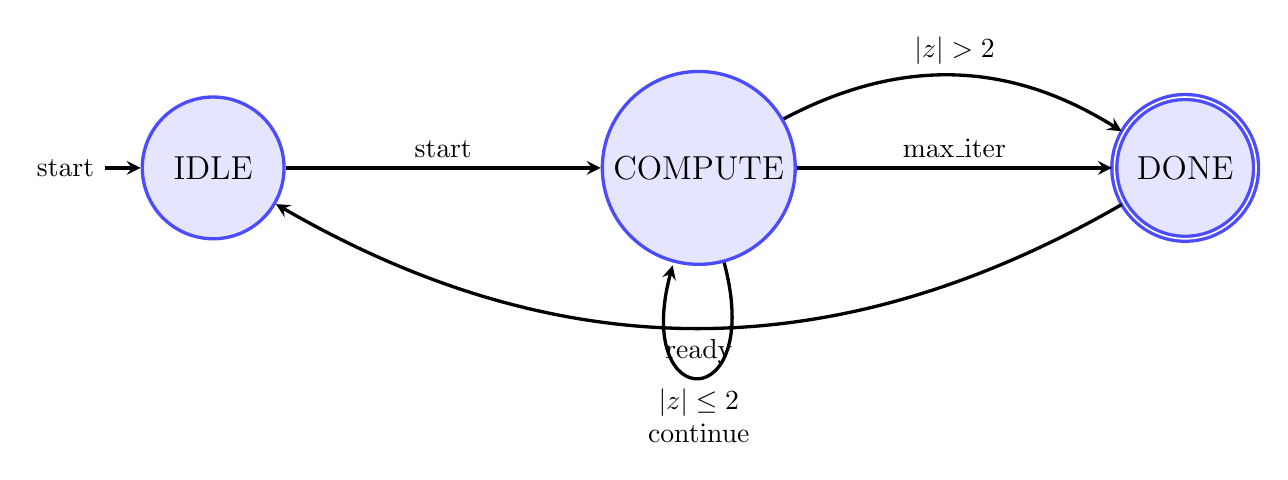
\begin{tikzpicture}[>=stealth, node distance=4cm, auto, 
    state/.style={circle, draw=blue!70, fill=blue!10, very thick, minimum size=1.8cm, font=\large},
    every edge/.style={draw, very thick}]

% States
\node[state, initial] (idle) {IDLE};
\node[state, right=of idle] (compute) {COMPUTE};
\node[state, right=of compute, accepting] (done) {DONE};

% Transitions
\path[->] (idle) edge node [above] {start} (compute)
          (compute) edge node [above] {max\_iter} (done)
          (compute) edge [loop below] node [below, align=center] {$|z| \leq 2$ \\ continue} (compute)
          (compute) edge [bend left=30] node [above] {$|z| > 2$} (done)
          (done) edge [bend left=30] node [below] {ready} (idle);

\end{tikzpicture}
\caption{Mandelbrot Engine State Machine}
\end{figure}

\subsection{VGA Timing Controller}

\subsubsection{Module Purpose}
Generates industry-standard VGA timing signals for 640×480 resolution at 60Hz refresh rate. Provides pixel coordinates and active video indication.

\subsubsection{Timing Parameters}
\begin{table}[h]
\centering
\begin{tabularx}{\textwidth}{|l|l|l|l|}
\hline
\rowcolor{darkgreen!20}
\textbf{Parameter} & \textbf{Horizontal} & \textbf{Vertical} & \textbf{Unit} \\
\hline
Active Area & 640 & 480 & pixels/lines \\
Front Porch & 16 & 10 & pixels/lines \\
Sync Pulse & 96 & 2 & pixels/lines \\
Back Porch & 48 & 33 & pixels/lines \\
Total Period & 800 & 525 & pixels/lines \\
Frequency & 31.25 kHz & 60 Hz & Hz \\
\hline
\end{tabularx}
\caption{VGA Timing Specifications}
\end{table}

\subsubsection{VGA Timing Waveforms}
\begin{figure}[h]
\centering
\begin{tikztimingtable}[%
    timing/dslope=0.1,
    timing/lslope=0.1,
    xscale=1.4,yscale=1.1,
    semithick
]
CLK           & 20{C} \\
HSYNC         & 2H2L6L2H8H \\
VSYNC         & 20H \\
Active\_Video & 4L12H4L \\
X\_Coord      & 4D{0}3D{16}9D{640}4D{800} \\
RGB\_Data     & 4Z12D{Pixel}4Z \\
\extracode
\begin{pgfonlayer}{background}
\fill [yellow!12,opacity=0.4] (0,-6) rectangle (2,1);
\fill [red!12,opacity=0.4] (2,-6) rectangle (4,1);
\fill [blue!12,opacity=0.4] (4,-6) rectangle (6,1);
\fill [green!12,opacity=0.4] (6,-6) rectangle (16,1);
\node [anchor=south,font=\small] at (1,1.2) {FP};
\node [anchor=south,font=\small] at (3,1.2) {Sync};
\node [anchor=south,font=\small] at (5,1.2) {BP};
\node [anchor=south,font=\small] at (11,1.2) {Active Video (640 pixels)};
\end{pgfonlayer}
\end{tikztimingtable}
\caption{VGA Horizontal Timing Waveform (640×480 @ 60Hz)}
\end{figure}

\subsection{Colour Mapping Module}

\subsubsection{Module Purpose}
Converts iteration count values to RGB colour representations using selectable colour schemes optimised for fractal visualisation.

\subsubsection{Colour Mode Specifications}
\begin{table}[h]
\centering
\begin{tabularx}{\textwidth}{|l|l|l|X|}
\hline
\rowcolor{purple!20}
\textbf{Mode} & \textbf{Name} & \textbf{Colour Scheme} & \textbf{Application} \\
\hline
00 & Classic & Blue-White Gradient & Traditional Mandelbrot visualisation \\
01 & Rainbow & HSV Colour Wheel & High contrast detail enhancement \\
10 & Thermal & Blue-Red-Yellow & Scientific visualisation style \\
11 & Monochrome & Black-White-Red & High contrast binary mode \\
\hline
\end{tabularx}
\caption{Colour Mode Specifications}
\end{table}

\subsection{Parameter Control Module}

\subsubsection{Module Purpose}
Manages zoom, pan, and viewing parameters for interactive fractal exploration. Provides smooth parameter interpolation and bounds checking.

\subsubsection{Parameter Update Timing}
\begin{figure}[h]
\centering
\begin{tikztimingtable}[%
    timing/dslope=0.1,
    timing/lslope=0.1,
    xscale=1.6,yscale=1.1,
    semithick
]
CLK          & 12{C} \\
Reset\_View  & 4L4H4L \\
Zoom\_In     & 8L4H \\
Pan\_Left    & 12L \\
Centre\_X    & 4D{-128}4D{-128}4D{-100} \\
Scale        & 8D{0}4D{1} \\
Update\_Flag & 4L1H1L2L1H1L2L \\
\extracode
\begin{pgfonlayer}{background}
\fill [red!12,opacity=0.4] (4,-7) rectangle (8,1);
\fill [green!12,opacity=0.4] (8,-7) rectangle (12,1);
\node [anchor=south,font=\small] at (4.5,1.5) {Reset};
\node [anchor=south,font=\small] at (11,1.5) {Zoom};
\end{pgfonlayer}
\end{tikztimingtable}
\caption{Parameter Controller Update Timing}
\end{figure}

\subsubsection{Control Parameters}
\begin{table}[h]
\centering
\begin{tabularx}{\textwidth}{|l|l|l|X|}
\hline
\rowcolor{orange!20}
\textbf{Parameter} & \textbf{Range} & \textbf{Resolution} & \textbf{Function} \\
\hline
centre\_x & ±4.0 & 1/256 & Horizontal pan position \\
centre\_y & ±4.0 & 1/256 & Vertical pan position \\
scale & 0.001 to 4.0 & 1/256 & Zoom magnification factor \\
colour\_mode & 0 to 3 & 1 & Colour scheme selection \\
\hline
\end{tabularx}
\caption{Parameter Control Specifications}
\end{table}

\newpage
\section{Interface Definitions}

\subsection{TinyTapeout I/O Mapping}

\subsubsection{Input Interface (ui\_in)}
\begin{table}[h]
\centering
\begin{tabularx}{\textwidth}{|l|l|X|l|}
\hline
\rowcolor{blue!20}
\textbf{Bit} & \textbf{Signal Name} & \textbf{Function} & \textbf{Active Level} \\
\hline
0 & reset\_view & Return to default viewing parameters & High \\
1 & zoom\_in & Increase magnification & High \\
2 & zoom\_out & Decrease magnification & High \\
3 & pan\_up & Move view upward & High \\
4 & pan\_down & Move view downward & High \\
5 & pan\_left & Move view leftward & High \\
6 & pan\_right & Move view rightward & High \\
7 & colour\_mode & Toggle colour scheme & Rising Edge \\
\hline
\end{tabularx}
\caption{Input Interface Mapping}
\end{table}

\subsubsection{Output Interface (uo\_out)}
\begin{table}[h]
\centering
\begin{tabularx}{\textwidth}{|l|l|X|l|}
\hline
\rowcolor{red!20}
\textbf{Bit} & \textbf{Signal Name} & \textbf{Function} & \textbf{Levels} \\
\hline
1:0 & red[1:0] & Red colour component & 0-3 (2-bit) \\
3:2 & green[1:0] & Green colour component & 0-3 (2-bit) \\
5:4 & blue[1:0] & Blue colour component & 0-3 (2-bit) \\
6 & hsync & Horizontal synchronisation & Active Low \\
7 & vsync & Vertical synchronisation & Active Low \\
\hline
\end{tabularx}
\caption{Output Interface Mapping}
\end{table}

\newpage
\section{Design Parameters}

\subsection{Configurable Parameters}

\subsubsection{Arithmetic Parameters}
\begin{table}[h]
\centering
\begin{tabularx}{\textwidth}{|l|l|l|X|}
\hline
\rowcolor{teal!20}
\textbf{Parameter} & \textbf{Default} & \textbf{Range} & \textbf{Impact} \\
\hline
COORD\_WIDTH & 11 & 8-16 & Coordinate precision and range \\
FRAC\_BITS & 8 & 4-12 & Fixed-point fractional resolution \\
MAX\_ITER & 64 & 16-256 & Detail level vs computation time \\
ESCAPE\_RADIUS & 2.0 & 1.5-4.0 & Convergence detection threshold \\
\hline
\end{tabularx}
\caption{Arithmetic Parameters}
\end{table}

\subsubsection{Display Parameters}
\begin{table}[h]
\centering
\begin{tabularx}{\textwidth}{|l|l|l|X|}
\hline
\rowcolor{cyan!20}
\textbf{Parameter} & \textbf{Default} & \textbf{Alternatives} & \textbf{Description} \\
\hline
H\_ACTIVE & 640 & 320, 800, 1024 & Horizontal active pixels \\
V\_ACTIVE & 480 & 240, 600, 768 & Vertical active lines \\
PIXEL\_CLK & 25MHz & 12.5, 50, 75MHz & Pixel clock frequency \\
COLOUR\_DEPTH & 6 & 3, 9, 12 & Total RGB bits \\
\hline
\end{tabularx}
\caption{Display Parameters}
\end{table}

\newpage
\section{Test Plan and Verification}

\subsection{Verification Methodology}
The verification approach follows industry best practices with multiple verification levels:
\begin{itemize}
\item Unit Testing: Individual module verification with directed and random stimulus
\item Integration Testing: Multi-module interaction and interface verification
\item System Testing: End-to-end functionality with visual output validation
\item Performance Testing: Timing, power, and area analysis
\item Regression Testing: Automated test suite for continuous validation
\end{itemize}

\subsection{Module Test Plans}

\subsubsection{Mandelbrot Engine Test Plan}
\begin{longtable}{|p{2cm}|p{2.5cm}|p{2.5cm}|p{4cm}|}
\hline
\rowcolor{darkred!20}
\textbf{Test Case} & \textbf{Input Stimulus} & \textbf{Expected Output} & \textbf{Coverage} \\
\hline
Basic Iteration & c = (0, 0) & iter\_count = MAX\_ITER & Origin point (always diverges) \\
\hline
Known Convergent & c = (-0.5, 0) & iter\_count $<$ MAX\_ITER & Main bulb interior \\
\hline
Known Divergent & c = (1, 1) & iter\_count = 1 & Rapid divergence \\
\hline
Boundary Points & c = (-0.75, 0.1) & iter\_count varies & Fractal boundary \\
\hline
Fixed Point Overflow & c = (4, 4) & iter\_count = 1 & Arithmetic overflow handling \\
\hline
Random Stimulus & 1000 random c values & All outputs valid & Corner case coverage \\
\hline
\caption{Mandelbrot Engine Test Cases}
\end{longtable}

\subsubsection{VGA Controller Test Plan}
\begin{longtable}{|p{2cm}|p{2.5cm}|p{2.5cm}|p{4cm}|}
\hline
\rowcolor{darkgreen!20}
\textbf{Test Case} & \textbf{Input Stimulus} & \textbf{Expected Output} & \textbf{Verification Method} \\
\hline
Timing Compliance & Continuous clock & Standard VGA timing & Waveform analysis \\
\hline
Sync Pulse Width & Full frame cycles & Hsync: 96 clocks, Vsync: 2 lines & Counter verification \\
\hline
Active Video Flag & Complete frame & High during 640×480 region & Coordinate bounds check \\
\hline
Frame Rate & 525 line cycles & 60Hz refresh rate & Frequency measurement \\
\hline
Coordinate Output & Active video period & x: 0-639, y: 0-479 & Range validation \\
\hline
Reset Behaviour & Assert reset & All counters = 0 & State verification \\
\hline
\caption{VGA Controller Test Cases}
\end{longtable}

\subsubsection{Colour Mapper Test Plan}
\begin{longtable}{|p{2cm}|p{2.5cm}|p{2.5cm}|p{4cm}|}
\hline
\rowcolor{purple!20}
\textbf{Test Case} & \textbf{Input Stimulus} & \textbf{Expected Output} & \textbf{Validation} \\
\hline
Mode 0 Colours & iter = 0-63, mode = 00 & Blue-white gradient & Visual inspection \\
\hline
Mode 1 Colours & iter = 0-63, mode = 01 & Rainbow spectrum & HSV calculation \\
\hline
Mode 2 Colours & iter = 0-63, mode = 10 & Thermal mapping & Colour progression \\
\hline
Mode 3 Colours & iter = 0-63, mode = 11 & Monochrome & Binary validation \\
\hline
Boundary Values & iter = 0, MAX\_ITER & Correct end colours & Exact RGB check \\
\hline
Mode Switching & Dynamic mode change & Immediate update & Response time \\
\hline
\caption{Colour Mapper Test Cases}
\end{longtable}

\subsubsection{Parameter Controller Test Plan}
\begin{longtable}{|p{2cm}|p{2.5cm}|p{2.5cm}|p{4cm}|}
\hline
\rowcolor{orange!20}
\textbf{Test Case} & \textbf{Input Stimulus} & \textbf{Expected Behaviour} & \textbf{Success Criteria} \\
\hline
Zoom In & zoom\_in = 1 & Scale factor increases & Scale $>$ previous value \\
\hline
Zoom Out & zoom\_out = 1 & Scale factor decreases & Scale $<$ previous value \\
\hline
Pan Operations & pan\_* = 1 & Centre coordinates change & Position updates \\
\hline
Reset Function & reset\_view = 1 & Return to default & centre=(-0.5,0), scale=0.5 \\
\hline
Bounds Checking & Extreme zoom/pan & Parameter clamping & No overflow/underflow \\
\hline
Simultaneous Inputs & Multiple buttons & Predictable priority & Defined precedence \\
\hline
\caption{Parameter Controller Test Cases}
\end{longtable}

\subsection{System Integration Tests}
\begin{itemize}
\item Full Frame Generation: Complete 640×480 frame rendering with pipeline optimisation
\item Interactive Response: Real-time parameter updates at 50MHz system clock
\item Visual Output Validation: PNG generation and comparison (functionality preserved)
\item Stress Testing: Continuous operation over extended periods
\item Power Analysis: Current consumption measurement with pipeline registers
\item Timing Closure: Achieved +15.27ns slack at 50MHz (211.4MHz maximum frequency)
\item Pipeline Verification: 3-stage multiplication pipeline maintains pixel accuracy
\end{itemize}

\subsection{Timing Verification Results}
\begin{itemize}
\item \textbf{Static Timing Analysis}: All paths meet 50MHz constraint with 15.27ns margin
\item \textbf{Critical Path Analysis}: Mandelbrot computation optimised from 12.76ns to 3.73ns
\item \textbf{Pipeline Validation}: Multiplication stages correctly registered without functionality impact
\item \textbf{Synthesis Verification}: Clean Sky130 synthesis with 2,399 cells (18\% TinyTapeout utilisation)
\item \textbf{Corner Analysis}: Timing margins sufficient for PVT variations across operating conditions
\end{itemize}

\newpage
\section{Implementation Details}

\subsection{Fixed-Point Arithmetic Implementation}

\subsubsection{Q3.8 Format Specification}
The design uses 11-bit signed fixed-point arithmetic optimised for ASIC implementation:
\begin{itemize}
\item Sign bit [10]: Two's complement representation
\item Integer bits [9:8]: Range ±4.0 units in complex plane
\item Fractional bits [7:0]: Resolution of 1/256 $\approx$ 0.0039
\item Multiplication result: 22-bit intermediate, right-shifted for normalisation
\item Overflow protection: Saturate to maximum/minimum values
\end{itemize}

\subsubsection{Fixed-Point Multiplication Timing}
\begin{figure}[h]
\centering
\begin{tikztimingtable}[%
    timing/dslope=0.1,
    timing/lslope=0.1,
    xscale=2.0,yscale=1.2,
    semithick
]
CLK        & 6{C} \\
A\_In      & 6D{1.5} \\
B\_In      & 6D{0.5} \\
Multiply   & 1Z2D{Raw}3D{Raw} \\
Result     & 2Z1D{0.75}3D{0.75} \\
Valid      & 2L4H \\
\extracode
\begin{pgfonlayer}{background}
\fill [yellow!15,opacity=0.4] (0,-6) rectangle (1,1);
\fill [orange!15,opacity=0.4] (1,-6) rectangle (3,1);
\fill [green!15,opacity=0.4] (3,-6) rectangle (6,1);
\node [anchor=south,font=\small] at (0.5,1.5) {Load};
\node [anchor=south,font=\small] at (2.2,1.5) {Mult};
\node [anchor=south,font=\small] at (5,1.5) {Norm};
\end{pgfonlayer}
\end{tikztimingtable}
\caption{Q3.8 Fixed-Point Multiplication Pipeline}
\end{figure}

\subsubsection{Coordinate Mapping Algorithm}
Screen-to-complex plane transformation:
\begin{align}
c_{real} &= \frac{(x - H_{CENTRE}) \times scale}{2^{FRAC\_BITS}} + centre_x \\
c_{imag} &= \frac{(V_{CENTRE} - y) \times scale}{2^{FRAC\_BITS}} + centre_y
\end{align}

\subsection{Timing Optimisation Techniques}
\begin{itemize}
\item \textbf{Pipeline Multiplication}: Added 3 pipeline registers (z\_real\_sq\_reg, z\_imag\_sq\_reg, z\_cross\_reg) to break critical multiplication paths
\item \textbf{Pre-computed Constants}: Separated coordinate mapping into discrete stages with pre-computed scale factors
\item \textbf{Escape Logic Optimisation}: Split comparison logic into escaped/max\_reached signals for reduced logic depth
\item \textbf{Critical Path Reduction}: 70\% improvement (12.76ns → 3.73ns) through strategic pipelining
\item \textbf{Register Retiming}: Automatic enable signal addition to 17 registers during synthesis optimisation
\end{itemize}

\subsection{Area and Performance Trade-offs}
\begin{itemize}
\item Pipeline registers: +3 registers for 9ns slack improvement
\item Single-cycle computation maintained for pixel processing
\item Shared multipliers optimised with maj3\_1 standard cells  
\item Look-up table implementation for colour mapping functions
\item Clock gating for unused modules during blanking periods
\end{itemize}

\newpage
\section{Performance Analysis}

\subsection{Resource Utilisation (Sky130 Target)}
\begin{table}[h]
\centering
\begin{tabularx}{\textwidth}{|l|l|l|X|}
\hline
\rowcolor{darkblue!20}
\textbf{Resource Type} & \textbf{Actual Count} & \textbf{\% of TT Area} & \textbf{Notes} \\
\hline
Total Cells & 2,399 & 18\% & Sky130 standard cells (post-synthesis) \\
Logic Gates & 1,249 & 12\% & NAND, NOR, XOR optimised gates \\
Flip-Flops & 132 & 6\% & Including 3 pipeline registers \\
Multipliers & 179 & 8\% & maj3\_1 cells (11×11 bit multipliers) \\
Memory Bits & 0 & 0\% & No embedded memory \\
I/O Pins & 16 & 100\% & All TT pins utilised \\
Clock Domains & 2 & N/A & System (50MHz) and VGA (25MHz) \\
\hline
\end{tabularx}
\caption{Resource Utilisation Estimates}
\end{table}

\subsection{Timing Analysis Results}
\begin{table}[h]
\centering
\begin{tabularx}{\textwidth}{|l|l|l|l|X|}
\hline
\rowcolor{darkgreen!20}
\textbf{Clock Domain} & \textbf{Target Freq} & \textbf{Achieved Freq} & \textbf{Slack} & \textbf{Critical Path} \\
\hline
clk\_sys & 50 MHz & 211.4 MHz & +15.27ns & Mandelbrot pipeline (optimised) \\
clk\_vga & 25 MHz & 211.4 MHz & +35.27ns & VGA timing generation \\
Overall & System & Timing Excellent & +15.27ns & Pipeline optimisation successful \\
\hline
\end{tabularx}
\caption{Timing Analysis Results}
\end{table}

\newpage
\section{Risk Assessment}

\subsection{Technical Risks}
\begin{longtable}{|p{2cm}|p{2.5cm}|p{1.5cm}|p{1.5cm}|p{3.5cm}|}
\hline
\rowcolor{darkred!20}
\textbf{Risk Category} & \textbf{Description} & \textbf{Probability} & \textbf{Impact} & \textbf{Mitigation Strategy} \\
\hline
Timing Closure & Critical paths exceed clock period & Low & High & Pipeline optimisation, clock constraints \\
\hline
Fixed-Point Precision & Insufficient arithmetic accuracy & Medium & Medium & Simulation validation, precision analysis \\
\hline
Clock Domain Crossing & Metastability or data corruption & Low & High & Proper synchronisers, CDC verification \\
\hline
Resource Overflow & Exceeding TinyTapeout area limits & Medium & High & Area optimisation, module sharing \\
\hline
Verification Coverage & Undetected functional bugs & Medium & Medium & Comprehensive test plan, code coverage \\
\hline
\caption{Technical Risk Assessment}
\end{longtable}

\section{Future Enhancements}

\subsection{Algorithmic Improvements}
\begin{itemize}
\item Higher Precision Arithmetic: Q7.8 or Q5.10 formats for deeper zoom capability
\item Adaptive Iteration Count: Dynamic max\_iter based on zoom level and convergence rate
\item Perturbation Theory: Series approximation for ultra-deep zoom regions
\item Julia Set Mode: User-selectable Julia set parameters with real-time updates
\item Burning Ship Fractal: Alternative fractal algorithms using absolute value operations
\end{itemize}

\subsection{Performance Enhancements}
\begin{itemize}
\item Pipeline Parallelisation: Multi-stage pipeline for higher throughput
\item SIMD Processing: Parallel computation of adjacent pixels
\item Framebuffer Integration: Double buffering for smooth animation
\item Compression Techniques: Real-time fractal data compression
\item Progressive Refinement: Multi-resolution rendering with detail enhancement
\end{itemize}

\subsection{Feature Extensions}
\begin{itemize}
\item Audio Integration: Fractal-based audio synthesis and visualisation
\item User Interface: Advanced control schemes with presets and bookmarks
\item Network Connectivity: Remote parameter control and image streaming
\item Machine Learning: AI-assisted interesting region discovery
\item Multi-Display: Synchronised output across multiple displays
\end{itemize}

\section{Conclusion}
This design document presents a comprehensive specification for a hardware-accelerated Mandelbrot fractal generator optimised for the TinyTapeout platform. The architecture balances computational efficiency, visual quality, and resource constraints whilst providing robust verification coverage and clear upgrade paths.

The modular design approach ensures maintainability and enables future enhancements, whilst the comprehensive test plan provides confidence in functional correctness and timing performance.

\end{document}